Using the sine formula, 
\begin{align}
 b\sin{C}=c\sin{B}
\\
\implies b\sin{90}=c\sin{30}
\\
\text{or, } c=2b
\end{align}
Similarly, 
\begin{align}
a\sin{B}&=b\sin{A}
\\
\implies a&=\sqrt{3}b
\end{align}
Formulating the above as a  matrix equation
\begin{align}
\myvec{0 & -2 & 1 \\1& -\sqrt{3}& 0 \\1& 1& 1&}\myvec{a\\b\\c} = \myvec{0\\0\\11}
\end{align}
Solving the above, 
\begin{align}
 a=4.026, b=2.32, c=4.64
\end{align} 
which are used to obtain the vertices
 of $\triangle ABC$ using Problem \ref{const:tri_sss}.  
\begin{align}
    \Vec{A}&=\myvec{0\\c}=\myvec{0\\4.64}\\\Vec{B}&=\myvec{0\\0}\\\Vec{C}&=\myvec{a\\0}=\myvec{4.02\\0}
\end{align}
The desired triangle is plotted in Fig. \ref{constr/9/fig:ABC}.
\begin{figure}[h!]
\centering
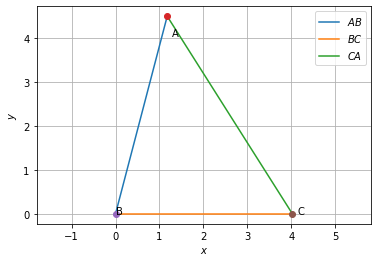
\includegraphics[width=\columnwidth]{solutions/9/figures/Figure11.png}
\caption{$\triangle ABC$}
\label{constr/9/fig:ABC}
\end{figure}